In this case, the SOC of the battery is set at 20\% as the initial SOC and the supercapacitor’s initial voltage is kept 170V with SOC of 25.2\%. These voltages are below acceptable limit. Steps similar to case 1 are also performed here.  At $t$ = 0.3s and $t$ = 0.6s, 34MW and 6MW load are connected to the MVDC system, respectively. At $t$ = 1s, 4MW pulsed load is added to the MVDC system and it is continued until $t$ = 2s. With the addition of pulsed load, the total load (44MW) of the system exceeds the total generation capacity (40MW). Considering those operations, it is expected that the FL controller based ESM system will provide the negative $P_{stor-ref}$ for discharging. But from Fig. \ref{ch5_f116}, the FL controller based ESM system provides zero $P_{stor-ref}$. This is because, the reference power generation by the FL controller based ESM system also depends on the SOC of the battery and supercapacitor ($SOC_{Bat}$, $SOC_{SC}$) with the other two input variables, $\Delta I$ and $V_{Bus}$. Due to low SOC (20\% and 25.2\%),  the FL controller based ESM system provides zero reference power. Simulation results after $t$ = 2s are the same as shown in case 1, where at $t$ = 2.5s, 4MW load is the battery and supercapacitor start charging and continue until $t$ = 3.5s.
\begin{figure}[ht!]
\begin{subfigure}{1\columnwidth}
\begin{center}
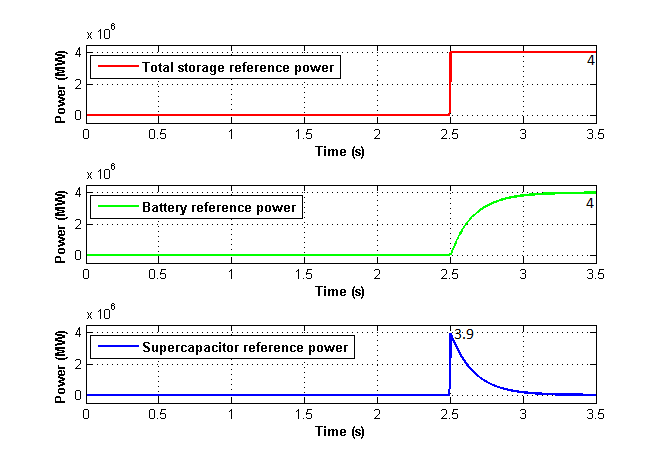
\includegraphics[height=3in, width=3.5in]{f116b}
\end{center}
\caption{Off-line simulation results.}
\label{ch5_f116b}
\end{subfigure}
\begin{subfigure}{1\columnwidth}
\begin{center}
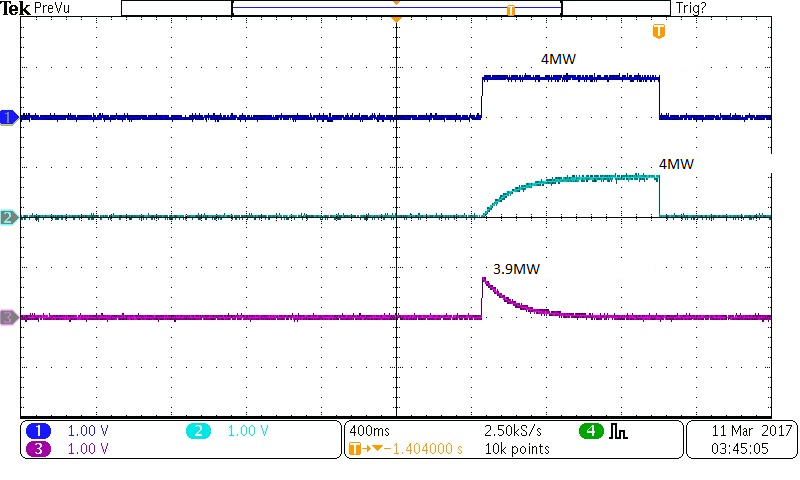
\includegraphics[height=2in, width=3.5in]{f116}
\end{center}
\caption{CHIL results-oscilloscope plots: Ch1: total storage reference power, Ch2: battery reference power, Ch3: supercapacitor reference  power (Ch1, Ch2, Ch3 = 5MW/div).}
\label{ch5_f116a}
\end{subfigure}
\caption{Reference power produced by FL controller and LPF based ESM system (case 2).}
\label{ch5_f116}
\end{figure}
